 
\chapter{Introduction}
\chapterauthor{Sebastian Nordhoff}{Max Planck Institute for Evolutionary Anthropology}

This book details the genesis of Sri Lanka Malay from a variety of angles. Before delving into contributions from typology, creole studies, Indian studies, Malay studies, historical demography and sociolinguistics, this introduction will  give an overview of the context of this fascinating language.

The Malays in Sri Lanka number about 50,000 people. Not all ethnic Malays are speakers of the language, and at present there is a noticeable shift from SLM towards English and Sinhala. The majority of the Malays live in the Colombo metropolitan area and in the smaller towns in the central Upcountry. Another important area is the southeastern coastal area, where we find the highest percentages of Malays on the island in the town of Hambantota (30\%) and the village of Kirinda (close to 100\%). The Malays -- with the exception of Kirinda --  are clearly an urban population, which is related to their close ties to the colonial administration.

\begin{figure}
\centering
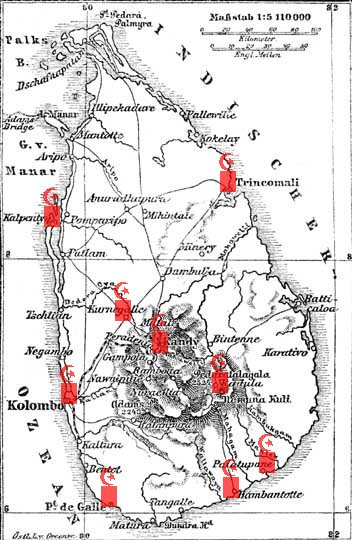
\includegraphics[height=.3\textheight]{\imgpath/m.jpg}
 \caption[Malay mosques during the colonial period]{Malay mosques during the colonial period. These are still indicative of the distribution of the Malay population today.}
\end{figure}



The Malays were mainly brought as soldiers during the Dutch (1656-1796) and British (1796-1948) rule of Ceylon, as the island was known then. The center of recruitment for the Dutch was Batavia on Java (today Jakarta). The recruits consisted of Javanese, Sundanese, Moluccans, Balinese, Buginese, and a variety of other peoples from the Indonesian archipelago. This group was complemented by royal exiles, convicts, and slaves. 
Looking at the ethnic makeup of the immigrant population, the term `Malay' is actually a misnomer. The Dutch referred to  them as `Javanen' or `Oosterlingen' (Easterlings). The connection with Java is also found in the Sinhala (\em jaa minissu\em) and Tamil (\em c\=avakar, j\=av\=a manusar\em) ethnonyms.
The immigrants came from a variety of ethnic backgrounds and spoke many different languages, but used Trade Malay as a lingua franca for interethnic communication. When the British took over from the Dutch in 1796, they noticed that this group spoke a variety of Malay, so they chose to call them `Malays', although almost none of them were ethnic Malays. The British continued recruiting in Jakarta until Indonesia was given back to the Dutch; the recruitment center shifted to the Straits Settlement then. It was only at this point in time that the first ethnic Malay immigrants came to Sri Lanka, but their linguistic varieties failed to have a significant impact \citep[see][]{Paauwtv}.

\begin{figure}
\centering
\subfigure[Dutch rule]{
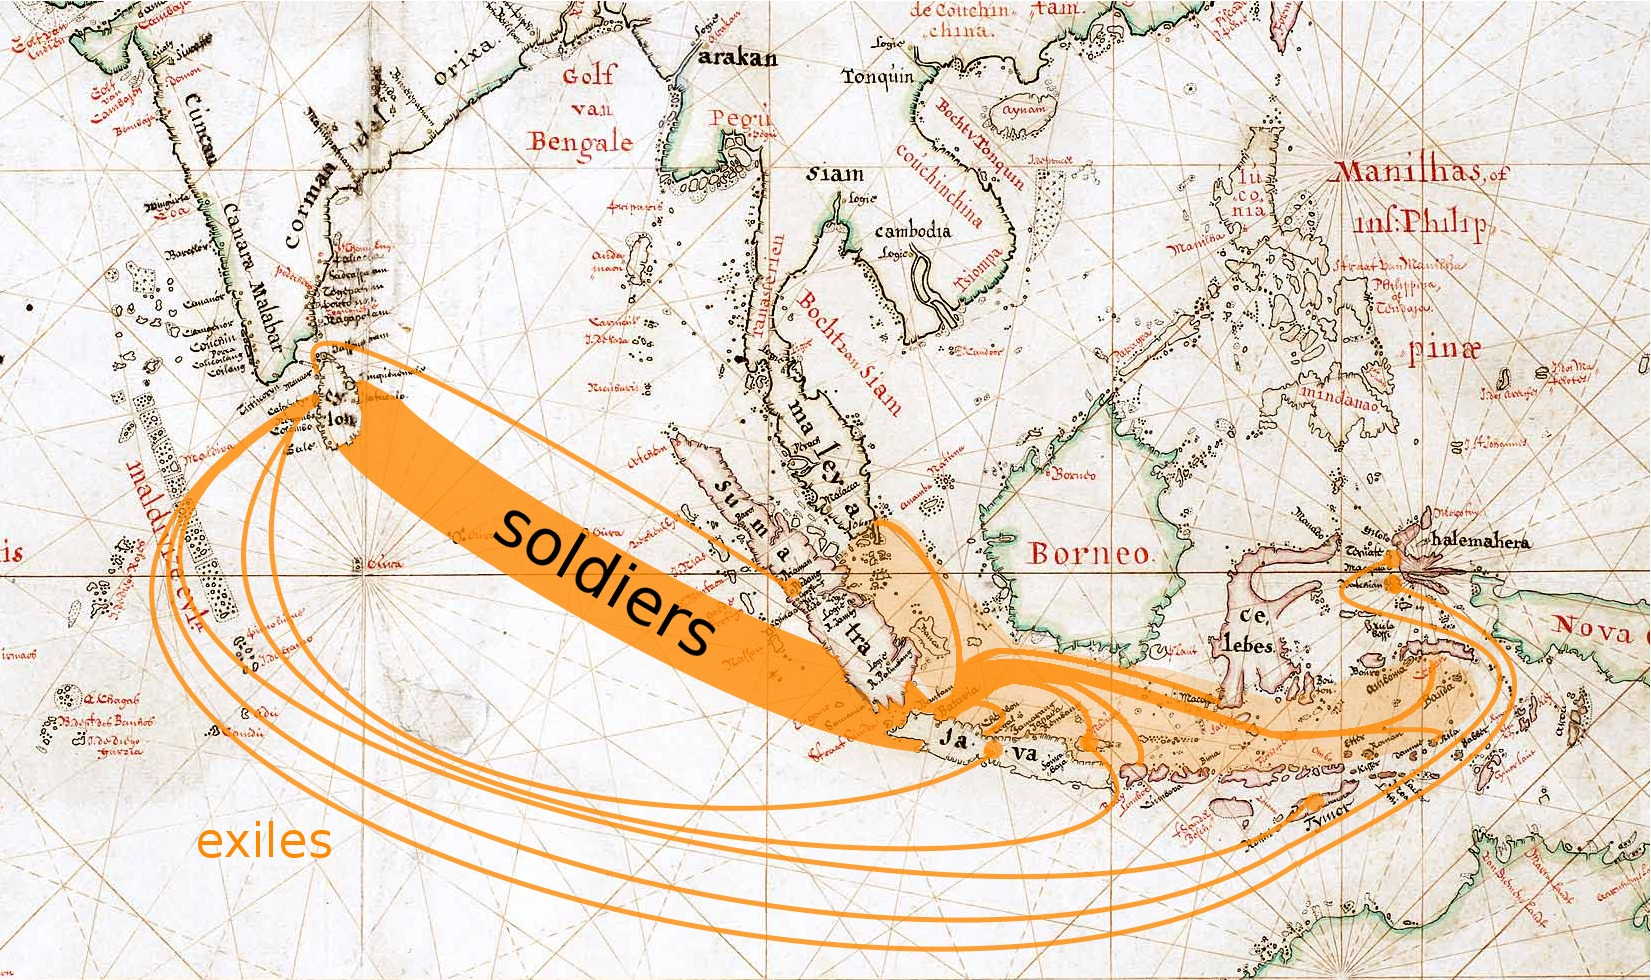
\includegraphics[width=\textwidth]{\imgpath/Dutchimmigration.jpg}
}
\subfigure[British rule]{
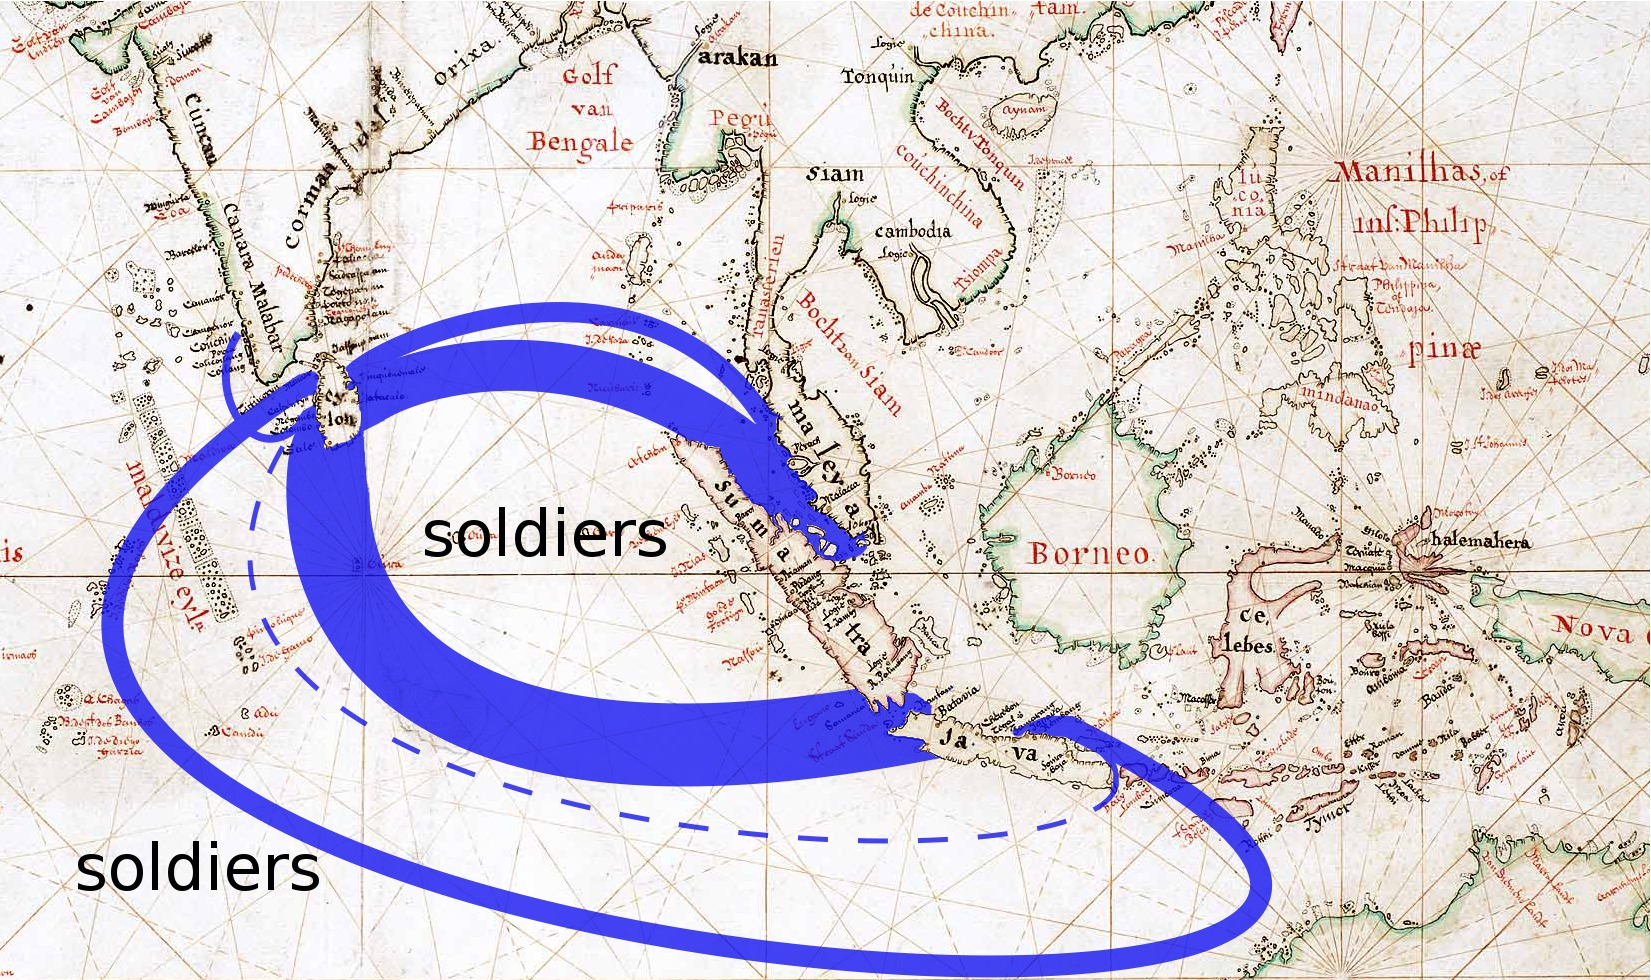
\includegraphics[width=\textwidth]{\imgpath/Englishimmigration.jpg}  
}
\caption{Migration during the colonial era.}
\end{figure}

Sri Lanka Malay culture is based on the military. The vast majority of immigrants were mercenaries, who fought in the jungle for the colonial powers, whose own soldiers were not fit for this climate and terrain. The braveness of the Malay soldiers is mentioned frequently, as is their addiction to gambling. 
 
Due to the large number of Malay soldiers, the British chose to set up  a special Malay regiment, which turned out to  be crucial for the development of Malay culture on the island \citep{Hussainmiya1987,Hussainmiya1990} as it provided the small group with the proximity and the close-knit network needed to maintain a vibrant diaspora community.  It is important to note that the 19th century Malays became the most educated of the native groups, second only to the Burghers (of European ancestry). After the disbandment of the regiment in 1873, the Malays kept their inclination towards the security  business and became policemen, firemen, overseers, or prison guards, but were dispersed all over the country. Their command of English remained much higher than that of the other groups due to their close ties with the colonial administration.

The turn of the century saw the rise of communalist tendencies among the Sinhalese, Tamil, and Moor populations, which led to the formation of a number of political organizations based on ethnicity. The Malays also set up their own  organization. It was at that time that the Malay hero, TB Jayah, joined the government and played a substantial role during the struggle for independence. Ceylon became independent from the UK in 1948. In 1956, the majoritarian Sinhalese population voted the Sinhala-Only law, which made schooling in Sinhala mandatory. The Malays had up to then used Sri Lanka Malay as the home language and English as the medium of schooling. Given that Sinhala replaced English in school, and that the Malays wanted to keep their comparatively better command of English, they opted for English as the home language. This meant that Malay was pushed out of the home domain, which is where the attrition of the language began. 


\begin{figure}
\begin{tabular}{lp{10cm}}
1503-1656& Portuguese rule \\
1656 & Start of Dutch rule  \\
-1700 & exiles from the Moluccas and the Lesser Sunda Islands; Java; and Bacan, Tidore, Timor, Madura, and Sumatra.  \\
17th and 18th c. & convicts, slaves \\
-1796 & soldiers (Ambonese, Bandanese, Balinese, Buginese, Javanese, Madurese, Malays)\\
1783 & existence of a Malay mosque in Sri Lanka\\
1796-1798 & British take over from the Dutch \\
-1816 & English recruit soldiers from Jakarta\\
1819- & English start recruiting on the Malaysian peninsula\\
1827 & foundation of the Ceylon Rifle Regiment \\
1873 & disbandment of the Regiment \\
1922 & foundation of the \textit{All Ceylon Malay Association}\\
1924 & Malays receive an appointed member of parliament \\
1948 & Independence of Ceylon\\
1956 & Sinhala Only Law\\
1965 & Malays lose their appointed member of parliament\\
1972 & Ceylon changes its name to Sri Lanka\\
1983 & start of the Sri Lankan Civil War \\
1985 & foundation of \textsc{slamac} (Sri Lankan Malay Confederation)\\
1989 & MH Amith is elected MoP for the Sri Lanka Muslim Congress \\
26 Dec 2004 & Tsunami \\
2009 & End of the Sri Lankan Civil War, rebels defeated\\
\end{tabular}
 \caption{Timeline of Sri Lanka Malay history.} 
\end{figure}


Ethnic upheaval between Tamils and Sinhalese followed the Sinhala-Only law and dominated the decades to come, eventually leading to the Sri Lankan Civil War (1983-2009). In this war, the Malays were loyal to the powers that be, i.e. the Sinhalese, and joining the army is still a common career choice for Sri Lanka Malays. Their command of Tamil was an asset in this domain, as they could be used behind enemy lines.

The 2004 Tsunami struck the community hard. Especially the coastal settlements of Kirinda, Hambantota and parts of Colombo were affected, with Hambantota paying the highest toll: about 1/3 of the Malay population there died on December 26, 2004.

The Upcountry was naturally not directly affected by this disaster, but was still shaken by the consequences of many friends and relatives' hardship.


Detailed sociological information about the Malays is lacking. They normally work in law enforcement and related areas or in white collar jobs. 
While \citet{Bichsel1989} refers to discrimination on the job market, unemployment does not seem to be a greater concern for the Malays today than for all Sri Lankans in general. Malays work as supreme court judges, national sportsmen, film stars, singers, media presenters, important journalists, or high representatives of Sri Lankan Airlines, so that we are not dealing with a systematic discrimination here. 
It is common to work for several years in the Gulf countries in order to earn enough money to buy a house. Sri Lankans generally live on their own property, or with their (extended) family.  

The Malays are Sunni Muslims and often have a very liberal interpretation of their faith. Marriage partners are either other Malays or members of the `Moor' group, who share their Islamic faith. Marriages to Sinhalese or Burghers do occur, but in these cases, the marriage partner is required to convert to Islam. Based on \citet{Nordhoff2009}, we can estimate that about 20\% of marriages are with Moors, but more thorough demographic research is required. 

The relationship to the Moors is a difficult one. On the one hand, both groups share the Islamic faith, on the other hand, the Malays tend to be  much more liberal and inclined towards education than the Moors, who have more traditional views and are more interested in commerce. The Malays resent the Moors' claim to speak for all Muslims ---The term `Muslim' is occasionally taken to mean `Moor'--- and find it important to mark the differences. As as result, the differences between Malays and Moors are occasionally highlighted and the commonalities tend to be played down.

The existence of Sri Lanka Malay was essentially ignored until the end of the 1980s, when \citet{Hussainmiya1987,Hussainmiya1990} and \citet{Bichsel1989} started publishing their work on the language. The 1990s saw some interest from senior European scholars \citep{Adelaar1991,Bakker1995nl,AdelaarEtAl1996}, and since the early years of this century, the study of Sri Lanka Malay can be regarded as established, both in the fields of Malay studies as well as in the field of contact linguistics.

While in the 20\textsuperscript{th} century, basic problems of description and social history were addressed, linguists working on the language in the 21\textsuperscript{st} century have focused on problems of genesis, where the relative importance of Tamil on the one hand and Sinhala on the other was the major point of contention. Ramifications of this debate include the existence and extent of intermarriage between Malays and Moors, the shape of the language in the early 19th century and the discussion which features could actually be used to determine the differential input from Sinhala and Tamil.

Sri Lanka Malay is very relevant for the field of contact linguistics because of a certain number of rare characteristics:
\begin{itemize}
 \item There is no Indo-European or West African input. This distinguishes it from most Creole languages.
 \item Sri Lanka Malay has mostly retained its lexicon but modified its grammar. This is the opposite of the  process of relexification often assumed for Creole genesis.
 \item Sri Lanka Malay became more complex during its development. It developed bound morphology such as non-finite forms and case markers absent in other varieties of Malay. Most theories predict that language contact should lead to simplification.
\item Sri Lanka Malay changed its grammar almost completely within only 300 years. This speed of development is extraordinary.
\end{itemize}


A schematic comparison between Sri Lanka Malay and the languages normally studied in creole studies is given in Table \ref{intro:tab:creoleslm}.

\begin{table}
\centering
\begin{tabular} {rll}
				&      Creole &      SLM \\
A language			&      +	&      + 	\\  
spoken\\
by displaced people		&   +  	&  +    	\\  
from Africa		&   (+)  	&   --   	\\  
on an island		&   (+)  	&   +   	\\  
in the tropics		&    + 	&  +    	\\  
who work for the colonizers		&  +   	&  +    	\\  
,who had forced their migration,		&  +   	&  (+)    	\\  
on plantations		&   +  	& --     	\\  
under appalling conditions		&  +   	&  --    	\\  
converting to Christianity		&  +   	&  --    	\\  
changing their original language		&  +   	&  +    	\\  
towards the colonizers' language		&  +   	& --     	\\  
retaining the grammar		&   +  	&  --    	\\  
and adopting the lexicon,		&   +  	&  --    	\\  
leading to a `simpler' language		&   +  	&  --    	\\  
within three to four centuries.		&   +  	&  +    	\\  
\end{tabular}
\caption{Comparison of a prototypical Creole setting with the Sri Lankan setting.}
\label{intro:tab:creoleslm}
\end{table}

In \xref{ex:intro:intro}, we see examples of the changes undergone by the language, comparing a simple sentence in Sri Lanka Malay with its Colloquial Indonesian translation.

\ea\label{ex:intro:intro}
\ea
\gll Saya tinggal di Colombo \textsc{Colloquial Indonesian}\\
      1\textsc{sg} live \textsc{loc} Colombo\\
`I live in Colombo.' (p.c. David Gil)
\ex
\gll Se Kluu{\umb}u=ka arà-duuduk \textsc{Sri Lanka Malay}\\
     1\textsc{sg} Colombo=\textsc{loc} \textsc{nonpast}-exist.\textsc{anim} \\  
      `I live in Colombo.'
\z
\z

We see that the order of constituents in the sentence is verb-medial in Indonesian but verb-final in Sri Lanka Malay. Similarly, Indonesian has a preposition \em di\em, where Sri Lanka Malay has a postposition \em=ka\em. This postposition is furthermore encliticized, showcasing the development of bound morphology in Sri Lanka Malay. Bound morphology can also be found in the verbal domain, where Sri Lanka Malay uses the obligatory prefix \em arà-\em, whereas tense marking in Indonesian is optional and often left omitted.  

In the domain of phonology, we can see the development of quantity distinction in the two vowels of \em duuduk \em and the phonemicization of prenasalised stops in \em Kluu{\umb}u\em. As for semantics, we can note the development of an animacy distinction in the existential, where animate \em duuduk \em  contrasts with  \em aada\em, which is underspecified for animacy. Both differ from \em tinggal \em as used in the Indonesian example. 

